\documentclass[_main.tex]{subfiles}
 
\begin{document}

\section*{Discussion}

Although the biology of parasite transmission dynamics is extremely complex, it is possible to summarise many of the fundamental processes in an idealised model with just three essential parameters: the quantum of transmission, the effective number of hosts and the crossing rate of transmission chains.  We have shown how this model, which we call the genomic transmission graph, lends itself to coalescent modelling and rapid simulation of different population genetic scenarios.  It also provides a mathematical framework for analysing within-host variation, and we show how this allows key parameters to be inferred from deep sequencing data.  

In this concluding section we discuss the practical relevance of these findings in the specific context of malaria biology and disease control.  Finally we consider the broader applications of the genomic transmission graph for recombining populations in general.

\paragraph{The quantum of transmission $Q$.}   Malaria parasites make a complex and arduous journey to get from host to host via a mosquito vector.  Only a tiny fraction of the billions of parasites carried by a human host finds its way into a mosquito vector, and fewer than 1\% of the sporozoites that develop within an infected mosquito find their way into the next human host on the transmission chain.  A wide range of transmission bottlenecks lie along this pathway including developmental roadblocks, specialised invasion mechanisms, host and vector immunity, and mosquito physiology and biting behaviour, as reviewed in reference \cite{Graumans2020}.

In our model, the quantum of transmission $Q$ represents the number of alleles that pass through this series of transmission bottlenecks in each cycle of host-to-host transmission. One way of estimating $Q$ would be to count the number of sporozoites that are inoculated by a mosquito into a new host, which in various experiments has been estimated to have a median value of 8 to 39 \cite{Graumans2020} but this is technically challenging to quantify directly, and it does not take account of other bottlenecks, e.g. the number of gametocytes taken up by the mosquito from the previous host.  

The value of $Q$ is crucial for understanding parasite cotransmission.  If $Q=1$ this means that only one allele is transmitted from one host to the next, hence we would expect to see a predominance of clonal infections.  Multiclonal infections arise due to superinfection and their recombinant progeny are propagated along the transmission chain.  As $Q$ increases it becomes increasingly likely that multiclonal infections will be cotransmitted from one host to the next.  If $Q$ is large, there could be many successive generations of cotransmission and recombination of multiclonal infections following a single episode of superinfection.

Here we describe a way of estimating $Q$ from measurements of within-host nucleotide diversity $\pi_W$ by deep genome sequencing.  Analysis of thousands of \textit{P. falciparum} samples from around the world reveals that the empirical distribution of $\pi_W$ is strikingly bimodal, and we postulate that one of the peaks ($\pi_W \approx 4 \times 10^{-7}$) comprises transmission chains that have not experienced superinfection in the recent past.  From equation \ref{eq:main_Q_est} this implies that $Q \approx 18$, which is reassuringly close to experimental estimates of the median number of sporozoites inoculated by an infectious mosquito, but this is a very preliminary estimate that requires more detailed analysis as described in Methods section \ref{supp_Q_pi}.

\paragraph{The crossing rate of transmission chains $\chi$.}  In regions of high transmission, malaria infections are often multiclonal, i.e. they contain multiple genetically distinct forms of the parasite.  Various methods have been developed to assess the number of distinct genetic forms of the parasite in a malaria-infected individual, known as the complexity of infection (COI) \cite{Thaithong1984,Viriyakosol1995,Galinsky2015,Chang2017}.  In the past it was widely assumed that the COI was a measure of how often an individual had been superinfected, but there is growing evidence - from single-cell sequencing \cite{Nkhoma2020}, deep sequencing \cite{Zhu2019} and epidemiological modelling \cite{Watson2020} - that multiclonal infections are often the result of cotransmission rather than superinfection.

In our model, the crossing rate of transmission chains $\chi$ represents the probability that a host is superinfected from two sources in one generation of the transmission graph. We do not explicitly model COI but it is implicit in our model that a relatively modest value of $\chi$ could lead to a high value of COI as long as the value of $Q$ is sufficiently high to allow cotransmission of multiclonal infections across multiple successive generations of the transmission graph.

From an epidemiological perspective, $\chi$ serves as a proxy measure of the incidence of infection.  More specifically, equation \ref{main:chi_tau} states that the incidence of infection is approximately equal to $\chi/ \tau$, where $\tau$ is the serial interval of infection, although this involves many simplifying assumptions.  

From a genetic perspective, $\chi$ determines the frequency of outcrossing in the population.  If $\chi = 0$ there is no outcrossing and the parasite population may appear to be clonal in nature, even though sexual recombination occurs with each generation of transmission between closely related sibling parasites.  If $\chi = 1$ there is a high rate of outcrossing, and in the special case of $\chi = 1$ and $Q = 1$ the genomic transmission graph is similar in many ways (but not identical) to a randomly mating diploid population. 

Here we describe a method of estimating $\chi$ from measurements of $F_{WS}$ by deep genome sequencing.  $F_{WS}$ is a metric that summarises the remarkably linear relationship that is observed between within-host heterozygosity ($\widehat{H}_W$) and the heterozygosity of the local subpopulation ($H_S$) when data are aggregated across hundreds of thousands of SNPs \cite{Manske2012}.  In equation \ref{eq:main_hwhs} we derive a formula that describes the slope of this linear relationship, and thus the value of $F_{WS}$, as a function of  $\chi$ and $Q$.  Analysis of $F_{WS}$ in thousands of samples indicates that $\chi \leq 0.1$ even in regions of high transmission where at least half of infections are multiclonal.  This supports the view that superinfection is much less common than cotransmission.

\paragraph{The effective number of hosts $N_h$.}  A key question in malaria epidemiology is the nature and size of the human infectious reservoir.  Only a small fraction of the hundreds of millions of people who are infected with \textit{P. falciparum} malaria annually \cite{WHO2022} go on to transmit parasites to a new host, and identifying those who are most likely to do so requires highly specialised and laborious epidemiological methods \cite{Goncalves2017}.  

It would be a major advance if parasite genetic data could be used to estimate the size of the infectious reservoir, and to determine how this varies over space and time following malaria control interventions.  In our model, $N_h$ represents the number of individuals that effectively transmit parasites to the next generation, and this might serve as a proxy measure for the human infectious reservoir.  

Effective population size ($N_e$) is a fundamental parameter of population genetics.  In theory it is the number of individuals that effectively contribute progeny to the next generation. In practice it is the estimated number of individuals required for an idealised population to reproduce genetic features observed in the real population.  $N_e$ is usually much smaller than the census population size, e.g. the ancestral effective population size of humans is on the order of magnitude of 10,000 individuals \cite{Henn2012}. 

Previous studies have estimated $N_e$ for \textit{P. falciparum} using a range of different approaches  \cite{Joy2003,Chang2012,Nkhoma2013,Anderson2017}.  The results are perplexing as they vary over several orders of magnitude depending on the method used, ranging from $10^2$ to $10^6$.  This problem is elegantly reviewed in reference \cite{Anderson2017}.  Some variation in $N_e$ is to be expected, depending on whether the population sampled is local or global, whether the methodology is designed to assess short-term or long-term $N_e$, and whether we are looking at rates of genetic drift or of adaptive evolution.  However the extreme variability observed in parasite $N_e$ implies that there is some fundamental problem in the application of classical population genetic methods to malaria \cite{Chan2013,Chang2015,Anderson2017}.  In our model we do not specify parasite $N_e$ but we know the size of the parasite population bottleneck which is given by $N_h Q$.  

There are a variety of ways by which $N_h$ might be estimated from empirical data (as is the case for $N_e$) giving different perspectives on the effective population size, e.g. short-term versus long-term and local versus global.  Here we illustrate the basic principles of a coalescent method of estimating long-term $N_h$ from the levels of nucleotide diversity observed in the global parasite population ($\pi_T \approx 4 \times 10^{-4}$).  Table \ref{table:comb_of_trans_var} shows various combinations of transmission parameters that would give this value of $\pi_T$, with $N_h$ ranging from 3,269 to 18,764 depending on the values of $Q$ and $\chi$.

\paragraph{Rate of migration $N_m$.}  Understanding patterns of migration of infected individuals is of basic importance in designing effective strategies for malaria elimination.  One way of thinking about this is in terms of a hierarchical population structure in which local subpopulations of parasites are interconnected parts of a global metapopulation.  In our model, the rate of migration $N_m$ represents the number of hosts that migrate each generation into a local subpopulation from the global (or regional) metapopulation.  Migration is also extremely important from a genetic perspective, as surprisingly low rates of $N_m$ can cause a small local subpopulation to acquire very nearly the same level of genetic diversity as the global metapopulation.  Here we present a simple model of migration across a hierarchical population structure that illustrates this point.

\paragraph{The effective reproduction number $R$.}  This key parameter of infectious disease transmission dynamics was conceived by Ronald Ross in his pioneering work on mathematical models of malaria over a hundred years ago \cite{Ross1915,Smith2012}.   In our model we do not specify $R$ but it is straightforward to estimate a reproduction number for $N_h$. Caution is needed in equating this with conventional epidemiological estimates of $R$ because $N_h$ represents the effective number of hosts that transmit parasites to the next generation and is probably much less than the total number of infected individuals.  As discussed above, we can view $N_h$ as a proxy for the human infectious reservoir, which may have different dynamical properties from the total number of infected individuals.

\paragraph{The effective recombination parameter $\phi_t$.}  In an insightful review, Camponovo and colleagues envisage how new statistical methods \cite{Kelleher2019,Speidel2019} will in future allow malaria transmission dynamics to be inferred from genome-wide ancestral recombination graphs that are much more informative on an epidemiological timescale than current mutation-based methods \cite{Camponovo2023}.  However they point out that this depends on the effective recombination rate which is affected by superinfection, cotransmission and population structure.

Here we provide a method of estimating the rate of effective recombination, which we define as recombination between heterozygous alleles that acts to change the DNA sequence of a haplotype locus.  By focusing on a haplotype locus, we allow for the possibility that recombination may be effective in some regions of the genome and not in others, particularly in the case of mating between genetically distinct but closely related individuals. 

In our model, the effective recombination parameter $\phi_t$ represents the probability that, if recombination occurs at a haplotype locus at time $t$, this will result in a change to the DNA sequence of that locus.  Thus the effective recombination rate is given by $\phi_t r L$ where $r$ is the locus-scaled recombination rate and $L$ is the length of the haplotype locus. 

The crucial insight is that $\phi_t$ is determined by the mean level of within-host heterozygosity in the population, and that this may vary over time.  Mating occurs within the vector but we make the simplifying assumption that within-host heterozygosity determines the probability that two mating alleles are genetically distinct, i.e. that they have different DNA sequences at a particular haplotype locus.  In equation \ref{eq:main_phi}, we let $\phi_t = f \widehat{H}_W$ where $f$ is a correction factor to allow for the possibility of mating bias and other confounders of the relationship between $\phi_t$ and $\widehat{H}_W$.

\paragraph{Identity by descent and recent common ancestry.}  \label{main_ibd_discussion}  

There is considerable interest in the use of IBD metrics to evaluate genetic relatedness between malaria parasites and to establish patterns of connectivity and recent migration betwen different geographical locations of malaria endemicity \cite{Schaffner2018,Henden2018,Taylor2017,Taylor2019,Taylor2020,Gerlovina2022}.  
 Conventional models of IBD count the number of meioses that separate two individuals, and estimate how segments of IBD are broken down by meiotic recombination assuming panmyxia, i.e. that mating occurs randomly across the population \cite{Browning2012}.  However malaria parasite populations are far from panmyctic because mating is rigidly compartmentalised into discrete within-host populations.  

By modelling the within-host population structure that arises from the parasite life cycle, the genomic transmission graph allows a more accurate view of the effective recombination rate.  In our model, shared haplotype segments of $>2$ centimorgans are essentially equivalent to segments of IBD, and the proportion of the genome that is IBD between two parasites can be crudely approximated by $\gamma$, the mean haplotype homozygosity of 2 centimorgan locus (figure \ref{fig:main_hap_hom_27}).  This provides a starting point for constructing a model of IBD that better reflects the parasite life cycle and thus allows more accurate inference of genetic relatedness. 

\paragraph{Using the transmission graph to infer epidemiological processes from genetic data.}  The work of Anderson and colleagues on the evolution of antimalarial drug resistance in Southeast Asia provides an elegant example of how longitudinally sampled genetic data, accompanied by rich epidemiological data, can be used in time series analysis to infer the parameters of a population genetic model \cite{Anderson2017}.  At the same time, their work highlights the limitations of current population genetic models as applied to malaria parasites, e.g. different types of genetic measurement give widely different estimates of effective population size.

The amount and the quality of time-series data on parasite genetic variation linked to rich epidemiological data will increase greatly over the next few years as genome sequencing becomes a routine part of malaria surveillance \cite{Inzaule2021}.  Epidemiological events - including fluctuations in population size, migration and transmission intensity - all shape the genetic architecture of the parasite population.   Our challenge is to infer those epidemiological events from genetic data, by understanding the causal relationship between epidemiological variables and genetic variables (figure \ref{fig:epi_mapping}).

The genomic transmission graph provides a theoretical model of this causal process, giving the mathematical relationship between a set of idealised transmission parameters and population genetic variables.  If we have rich epidemiological data coupled to genetic data from the same locations, ideally sampled over space and time, we can look for a correlation between the transmission parameters and the epidemiological variables.  We do not expect the idealised transmission parameters to represent exact values of any epidemiological variables, but we hope to find a sensible and reliable set of correlations that allow us to estimate the epidemiological variables from the transmission parameters and hence from the genetic data. 

\begin{figure}[h!]
\centering
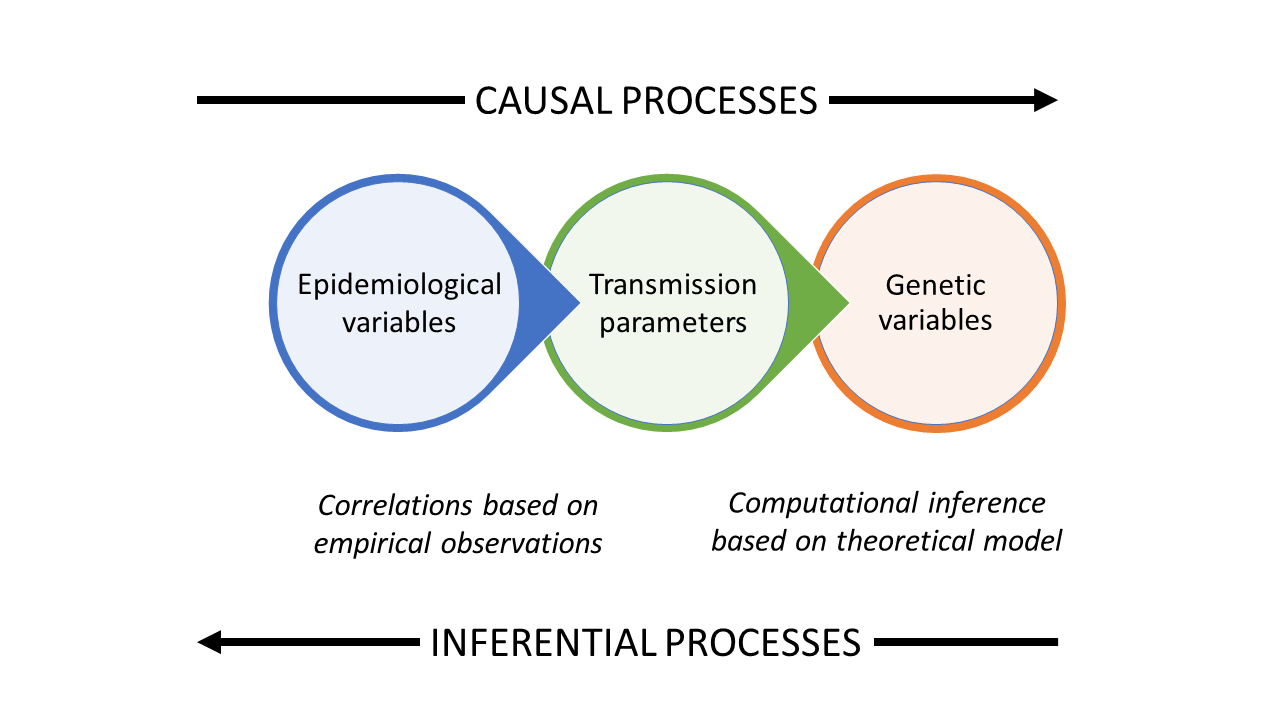
\includegraphics[width=14cm]{230120_inferential_processes.png}
\caption{\textbf{How epidemiological events can be inferred from genetic data.}  First the genetic data are used to make estimates of transmission parameters based on the mathematical relationships specified by the theoretical model of the transmission graph.  Then the epidemiological variables are inferred from the transmission parameters using a set of correlations and mappings that have been built up by many empirical observations.}
\label{fig:epi_mapping}
\end{figure}

\paragraph{Natural selection.}  It is conventional to focus on selectively neutral loci when using genetics to infer population dynamics, where the key processes of interest are mutation and genetic drift.   Therefore in our current model we ignore natural selection and adaptive evolution although these play a major role in shaping parasite genetic variation, particularly at drug resistance loci but also more generally across the genome \cite{Anderson2017,Amato2018,Band2022}.   

Natural selection can operate through many different mechanisms on a wide range of time scales.  The malaria life-cycle involves repeated cycles of rapid population expansion - of clonally replicating parasites within the host and of sexually reproducing parasites within the vector - punctuated by tight transmission bottlenecks.  This acts both to intensify natural selection and to obscure classic population genetic signatures of selection \cite{Chan2013,Chang2015}.  

Of particular interest for epidemiological monitoring is recent positive selection of new forms of drug resistance.  With modern methods of genetic epidemiology, it is often possible to identify the causal mutation of drug resistance and to measure its rising frequency in the population, i.e. to observe the selective sweep \cite{Anderson2017,Amato2018}.  In principle it would be possible to extend the current model to describe the selective sweep of a drug resistance locus using a structured coalescent approach, but that is beyond the scope of the current paper.

\paragraph{Limitations of the model.}  The genomic transmission graph is a deliberately simplistic model that sets aside many details in order to gain a clear view of fundamental mechanisms.  It seeks to elucidate how a small set of key transmission parameters - $Q$, $\chi$, $N_h$ and $N_m$ - act individually and in combination to shape parasite genetic diversity and population structure.  Its utility as a tool for learning about fundamental processes underlying genetic variation is greatly enhanced by its amenability to coalescent simulation which stems from the simple structure of the model.

This approach has obvious limitations, some of which would be relatively straightforward to address in modified versions of the model, e.g. we assume that parasites are transmitted from host to host in non-overlapping generations of fixed duration, which is clearly over-simplistic and might be improved by using a continuous-time Moran model \cite{Hendry2021}.  As another example, the current model allows superinfection from only two sources, but in principle we could allow any number of sources of superinfection by making $\chi$ a random variable.

Other limitations are more complex to address, e.g. we take no account of acquired immunity, antimalarial drug usage, vector biting behaviour and many other sources of heterogeneity in the host, parasite and vector populations.   In principle this could be addressed by incorporating the basic principles of the genomic transmission graph into agent-based epidemiological models that explictly deal with the details of malaria transmission biology, at the cost of introducing a large number of parameters that might be difficult to ascertain with confidence (and without overfitting the model) from available empirical data \cite{Eckhoff2012,Daniels2015,Griffin2016,Watson2020}.

\paragraph{Broader applications of the genomic transmission graph for recombining populations.}  Although this paper focuses on malaria, the transmission graph has wider implications for other parasites and for recombining populations in general.  In the case of malaria, each node of the graph represents the parasite subpopulation carried by an individual host, but more generally we can think of this as a transient subpopulation, i.e. a discrete group of individuals that exists at a certain point in time.  Framed in this general manner, each node of the graph represents a discrete group of individuals that undergo recombination before propagating along the edges of the graph to form one or more new groups.  The transmission graph describes the effective number and size of these groups and the rate at which they form new groups, merge with other groups, migrate between locations, or disappear.  With suitable modification, the genomic transmission graph might be useful for studying the evolutionary dynamics of other species that naturally cluster into many small groups that are continually propagating, merging and migrating, such as shoals of fish, flocks of birds or herds of animals.  It could also possibly be used for analysis of viral and bacterial species that undergo horizontal gene transfer when they congregate within individual hosts or other transient ecological niches. 

\end{document}